\chapter{The outline of the~method}\label{chap:outline}

\newcommand{\objnorm}[2]{\mathbold{#1_{#2}}}
\newcommand{\objdot}[2]{\mathbold{#1_{#2}^\bullet}}
\newcommand{\lnorm}[1]{\objnorm{L}{#1}}
\newcommand{\ldot}[1]{\mathbold{L_{#1}^\bullet}}

\newcommand{\opnorm}[2]{\mathit{#1_{#2}}}
\newcommand{\dnorm}{\opnorm{Q}{D}}

In this chapter, we will briefly describe how the~compression works. The~details of it are described in the~following Chapter~\ref{chap:details}. Basically, two consecutive passes are performed on the~input heightmap --- a~bottom-up pass followed by a~top-down pass (Fig.~\ref{fig:main_schema}). These passes are analogic to the~passes of the~described second-generation wavelet methods. 
	
	\begin{figure}
		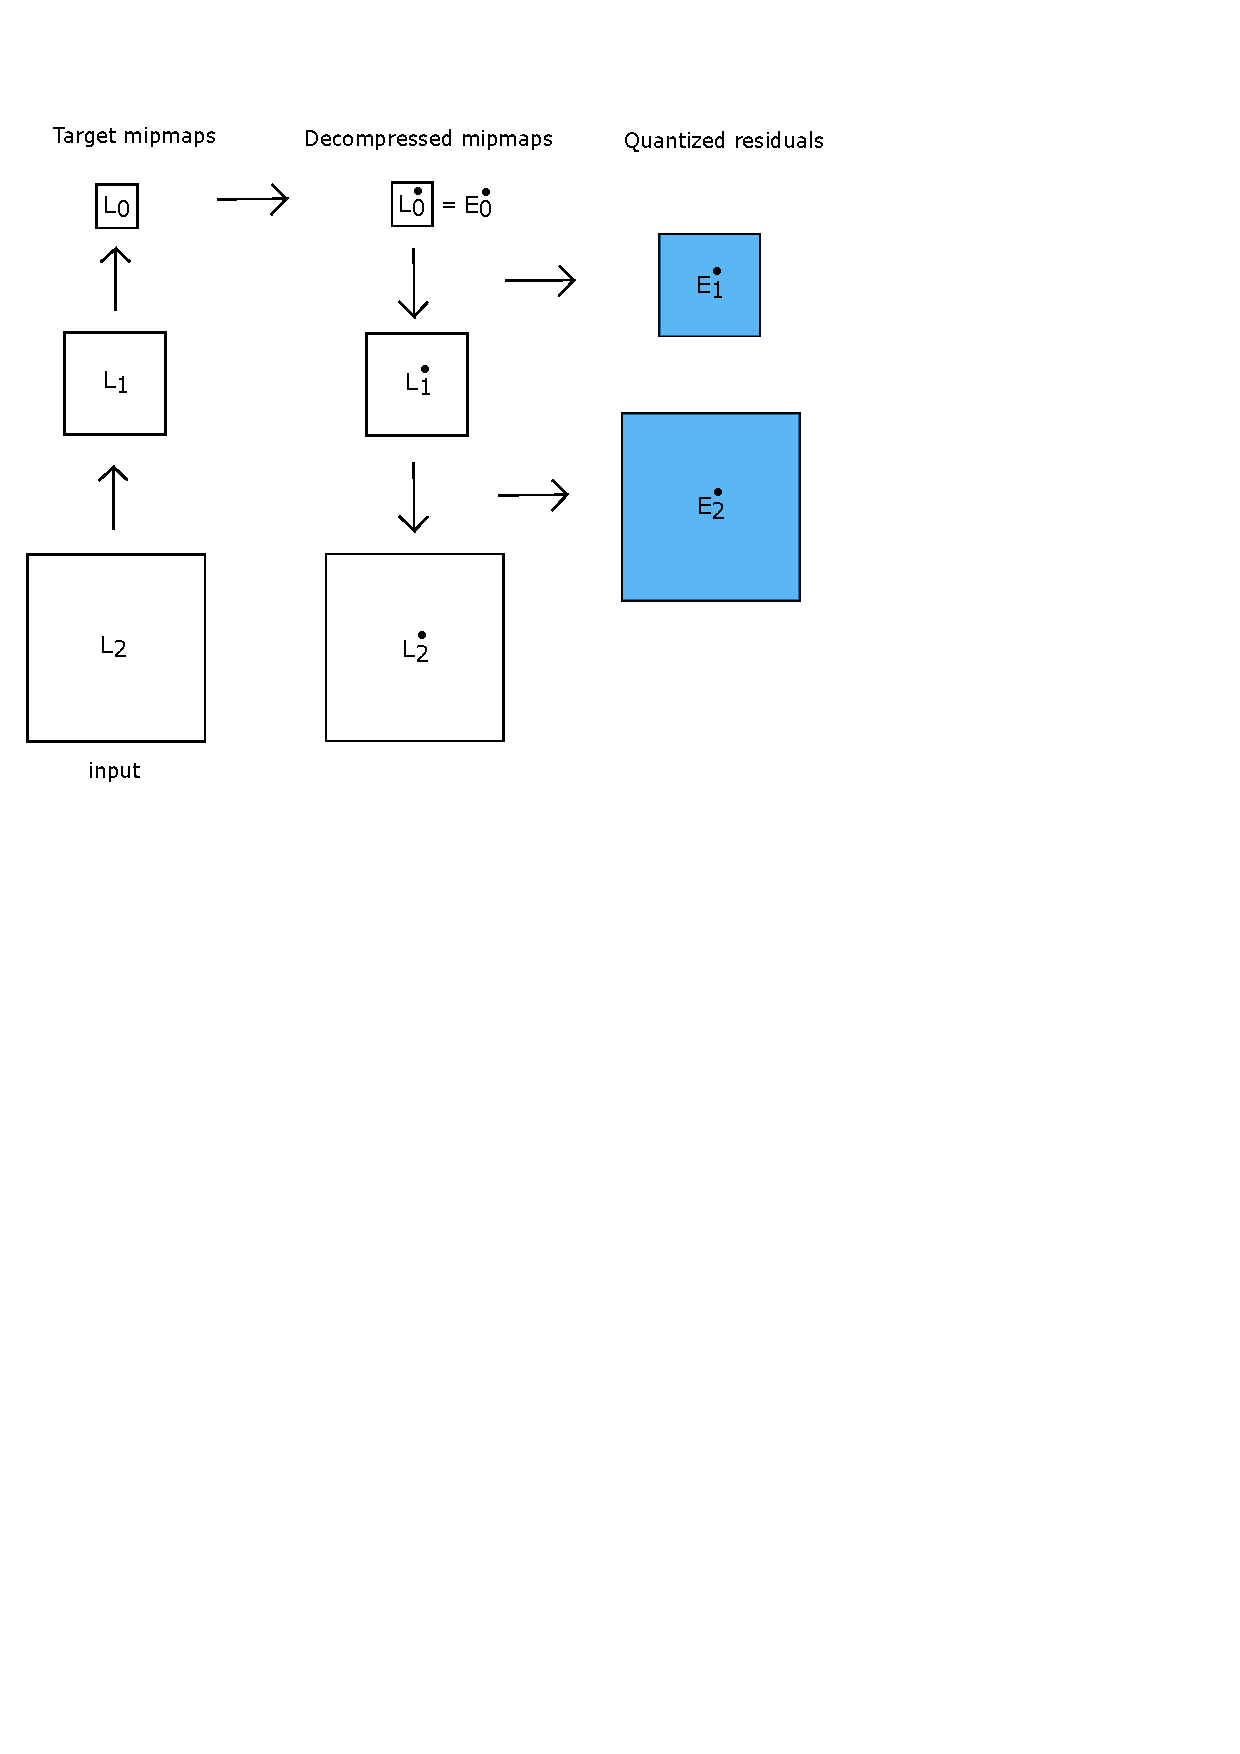
\includegraphics[trim={0 15cm 6cm 1cm}, clip, width=1\textwidth]{figures/main_schema.pdf}\centering
		\caption{The~main schema of compression of the~method. On the~left, the~target mip-maps $\lnorm{n}$ are constructed in the~first bottom-up pass. On the~right, the~decompressed mip-maps $\ldot{n}$ are constructed with respect to the~target mip-maps in the~second top-bottom pass. Each constructed mip-map is predicted from the~previous one and subtracted from the~neighbor target mip-map to obtain the~residuals which are then quantized to $\objdot{E}{n}$ and compressed.}
		\label{fig:main_schema}
	\end{figure}

The~first bottom-up pass computes the~target mip-maps --- from the~largest one to the~smallest one. Those will be the~mip-maps, against which the~accuracy of reconstruction will be measured. The~largest mip-map is the~input itself. Every smaller mip-map is computed from the~previous larger one. These mip-maps will be used just as a~temporary reference during compression and are not stored in any way.

The~second top-down pass then performs the~compression of these reference mip-maps. To explain how it works, let us firstly describe the~main idea of decompression: once we have a~certain decompressed mip-map, we can reconstruct the~following twice as large  decompressed mip-map with some additional information (residuals). This is quite convenient, as the~previous mip-map represents the~same terrain block, just in a~worse resolution, so the~residuals will be small most of the~time, and thus well compressible. Thus, in order to perform the~decompression, we just need to know the~first mip-map and all the~residuals. 

Now, let us get back to the~compression. It computes, quantizes, compresses and stores these residuals. However, in this process, it also computes the~decompressed mip-maps aside, so that right before the~computation of the~residuals needed to reconstruct a~mip-map from the~previous smaller one, the~smaller one is already known (Fig.~\ref{fig:main_schema}). This way, it is guaranteed that the~compression works with the~same mip-maps as the~decompression.  This is very important in order to be able to guarantee a~certain maximum deviation of each decompressed mip-map from its corresponding target mip-map. During the~compression, the~residuals are computed with respect to the~corresponding target reference mip-map from the~first pass, so that the~deviation of the~resulting decompressed mip-map is within the~bound. Thanks to the~fact that these residuals will be combined with the~same mip-map during the~decompression, the~resulting larger mip-map will also be the~same as the~one constructed during the~compression, conforming to the~maximum-error bound.

Now we will decribe the~mip-map refinement in a~bit more detail. Each mip-map except the~smallest one is firstly predicted from the~previous decompressed mip-map. These predictions are then subtracted from the~corresponding same-sized target mip-map to obtain the~residuals. These residuals are then quantized in such way that the~maximum deviation of the~current decompressed mip-map is still respected. Then, they are losslessly compressed and stored (Fig.~\ref{fig:single_reconst}). In the~decompression, the~fetched and decompressed residuals are just added to the~predictions to obtain the~finer mip-map (Fig.~\ref{fig:single_decomp}). Note that this method is lossless only due to the~quantization. If we omit this quantization, we the~method becomes lossless. This happens when the~maximum height deviation is set to 0 by the~user.

\begin{figure}
	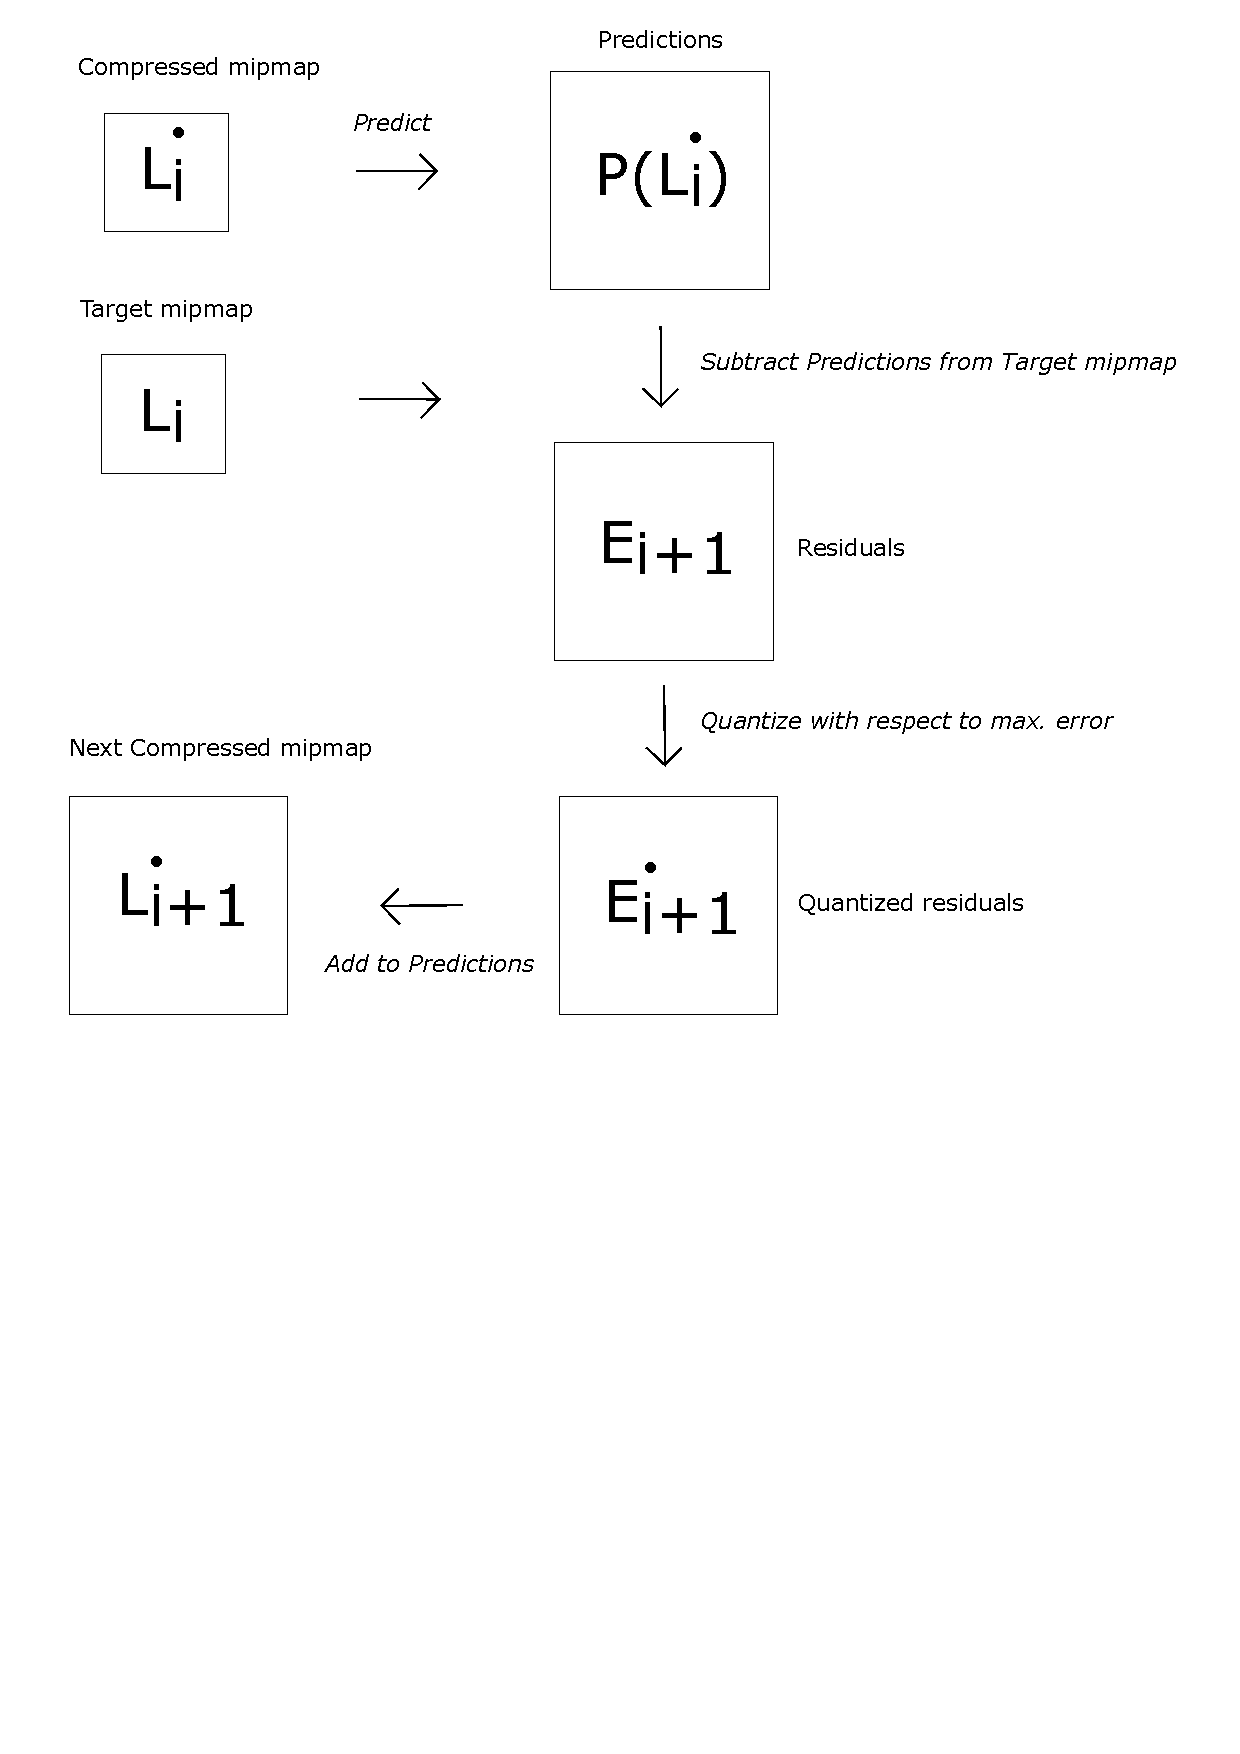
\includegraphics[trim={0 12cm 1cm 0cm}, clip, width=1\textwidth]{figures/single_reconst.pdf}\centering
	\caption{The~diagram of construction of larger decompressed mip-map $\ldot{i+1}$ from the~smaller $\ldot{i}$ during the~off-line compression. Only the~quantized residuals $\objdot{E}{i+1}$ are losslessly compressed and stored. They are sufficient to reconstruct $\ldot{i+1}$ from $\ldot{i}$.}
	\label{fig:single_reconst}
\end{figure}

\begin{figure}
	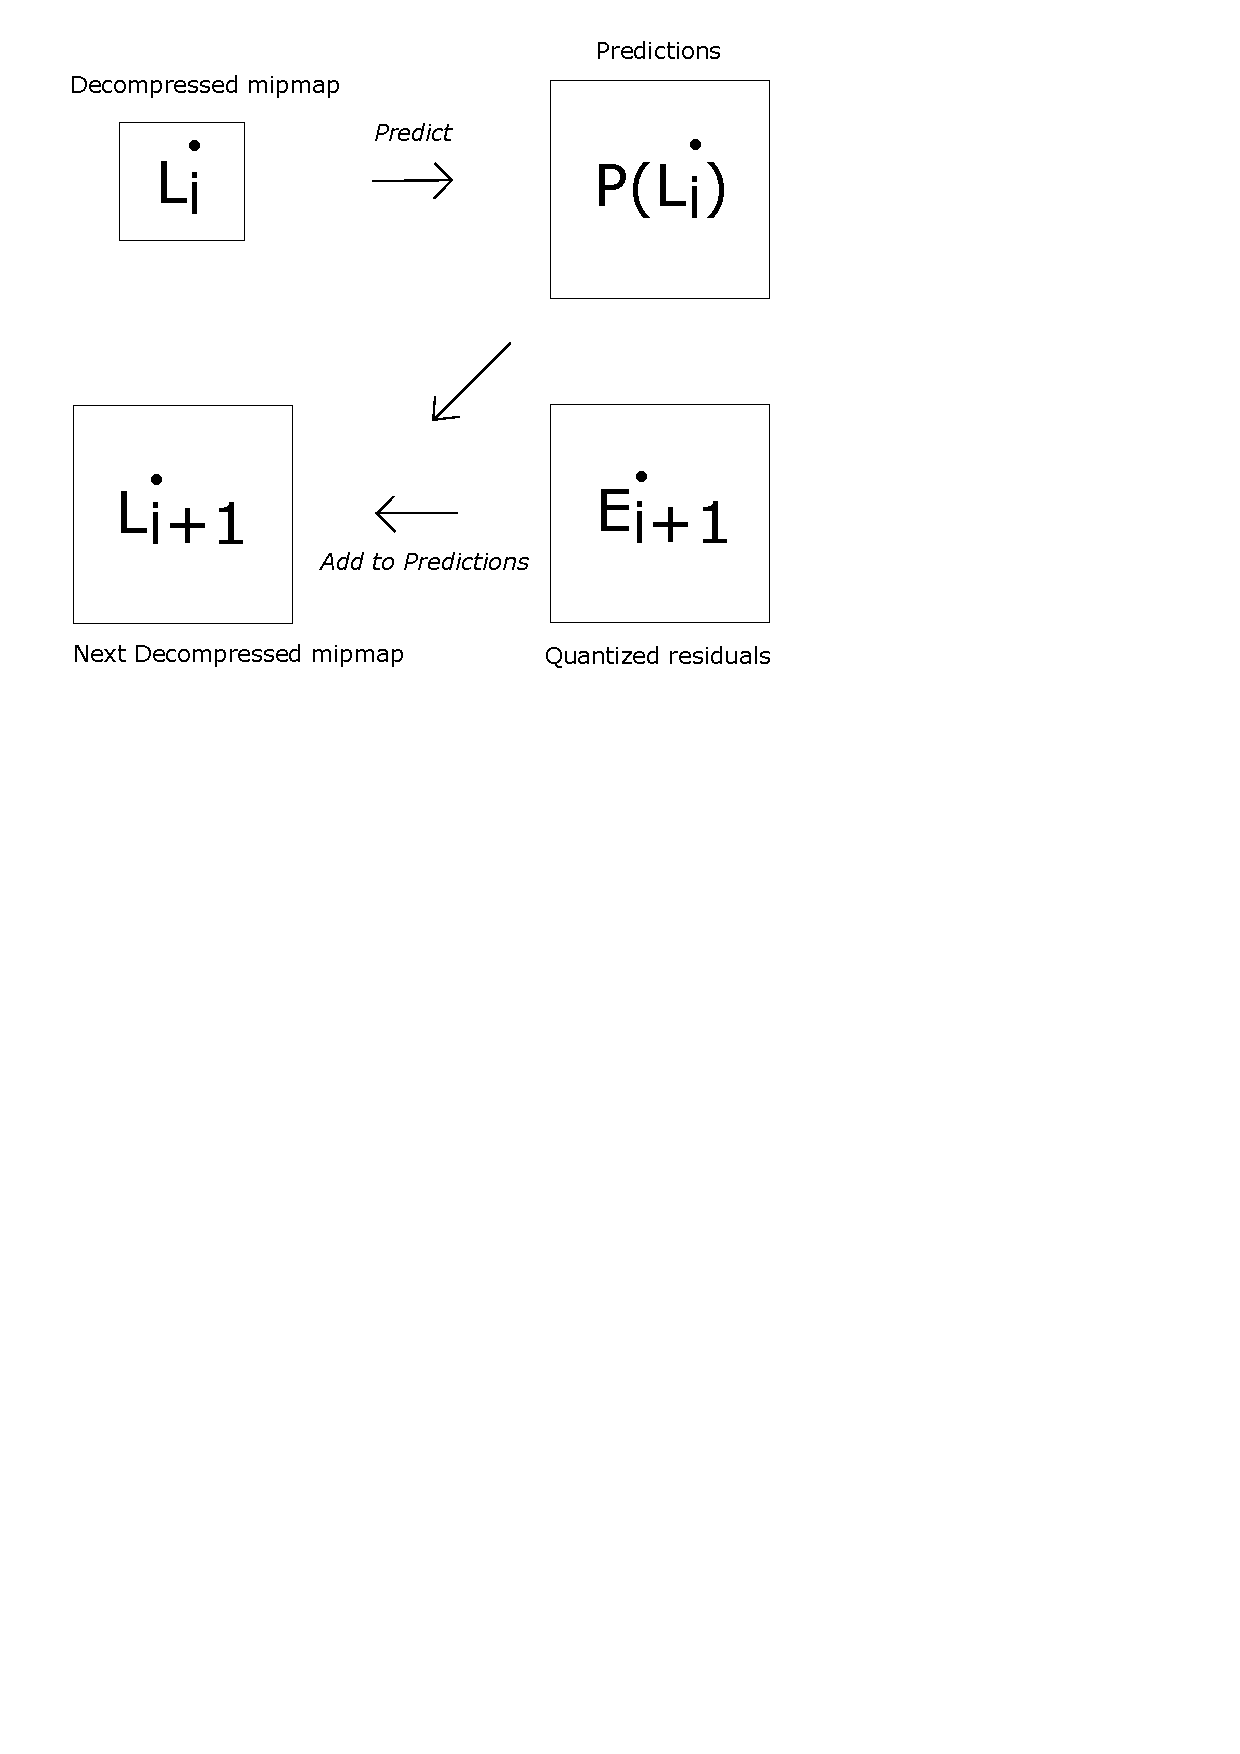
\includegraphics[trim={0 12cm 1cm 0cm}, clip, width=1\textwidth]{figures/single_decomp.pdf}\centering
	\caption{The~diagram of construction of larger decompressed mip-map $\ldot{i+1}$ from the~smaller $\ldot{i}$ during the~real-time decompression. The~quantized residuals $\objdot{E}{i+1}$ are read and decompressed. Then, they are added to the~predictions from the~smaller mip-map.}
	\label{fig:single_decomp}
\end{figure}

More formally, the~first pass is given the~input square block of float height samples $\lnorm{n}$ sized $2^n \times 2^n$ and produces $n$ mip-maps $\lnorm{n-1..0}$ from it, one by one. The~dimension of $\lnorm{i}$ is half the~dimension of $\lnorm{i+1}$. Just like it is common in mip-maps $\lnorm{i}$ is computed from $\lnorm{i+1}$ by straightforward averaging of pixels --- see the~details in the~following chapter. 

The~second top-down pass has already $\lnorm{0..n}$ available and computes $\ldot{0..n}$ --- the~decompressed mip-maps. The~dimension of $\lnorm{i}$ and $\ldot{i}$ is the~same. The~computation ensures that the~maximum absolute deviation between their~corresponding samples is not greater than $\objnorm{D}{}$ --- the~parameter set by the~user. This will be denoted by:
$$maxdev(\lnorm{i}, \ldot{i}) \leq \objnorm{D}{},$$
where
$$maxdev(A, B) = \underset{x, y}{\arg\max}|A[x][y] - B[x][y]|$$
We will achieve this with the~help of the~uniform quantizer $\opnorm{Q}{D}$ the~quantization step of which is set to the~maximum value which still respects this error bound:
$$maxdev(\dnorm(x), x) \leq \objnorm{D}{},$$
where $x$ is an arbitrary float sample or block of samples.
The~quantizing step of this quantizer is $2\objnorm{D}{} - 1$ in case $\objnorm{D}{} \geq 0.5$ and $2\objnorm{D}{}$ otherwise.


As we already mentioned, $\ldot{0}$ is just the~quantized sole value of $\lnorm{0}$:
$$\ldot{0} = \dnorm(\lnorm{0})$$
Thanks to the~fact that the~quantizer respects the~maximum-error bound $\objnorm{D}{}$, $maxdev(\lnorm{0}, \ldot{0}) \leq \objnorm{D}{}$.


Then, the~values of every following $\ldot{i+1}$ are predicted from the~values of the~previous $\ldot{i}$. The~raw differences between the~target values and the~predicted values are denoted as $\objnorm{E}{i+1}$ (the~residuals). With the~help of them and the~predictions from $\ldot{i}$, we would be able to accurately reconstruct the target mip-map $\lnorm{i+1}$. However, these residuals are then quantized with the~uniform quantizer $\opnorm{Q}{D}$ to $\objdot{E}{i+1}$. With the~help of the~quantized residuals, we are no longer able to accurately reconstruct $\lnorm{i+1}$, but thanks to the~fact that the~used quantizer keeps the~maximum absolute error within the~bound $\mathbold{D}$, we can guarantee that the~reconstructed $\ldot{i+1}$ will satisfy the~maximum-error constraint: $maxdev(\ldot{i+1}, \lnorm{i+1}) \leq \objnorm{D}{}$. Here is how we construct $\ldot{i+1}$:

$$\objnorm{E}{i+1} = \lnorm{i+1} - \opnorm{P}{}(\ldot{i})$$
$$\objdot{E}{i+1} = \opnorm{Q}{D}(\objnorm{E}{i+1})$$
\begin{equation}
\label{eq:nextLevel}
\ldot{i+1} = \opnorm{P}{}(\ldot{i}) + \objdot{E}{i+1}
\end{equation}

Thanks to the fact that the~residuals $\objnorm{E}{i+1}$ are computed with respect to the~target mip-map $\lnorm{i+1}$, the~maximum-error constraint is satisfied, no matter what values are in $\ldot{i}$ and what the~prediction operator $\opnorm{P}{}$ looks like. At the~end, the~quantized residuals $\objdot{E}{0..n}$ are losslessly compressed with the~help of Zlib and stored ($\objdot{E}{0} = \ldot{0}$). The~order of their storage is from $\objdot{E}{0}$ to $\objdot{E}{n}$, so that progressive decompression is possible. The~more accurate $\opnorm{P}{}$ is, the~smaller the~residuals are, thus the~higher the~compression ratio is. The~details of the~prediction operator used in this method are described in the~following chapter. The~higher $\objnorm{D}{}$ is, the~less entropy there is among the~residuals, thus the~higher the~compression ratio is, but the~lower the~reconstruction quality is.

The~real-time decompression then just reads the~stored quantized residuals and decompresses them with the~help of the~same lossless codec. Thanks to the~fact that the~residuals of a~smaller mip-map are stored before the~residuals of a~larger mip-map, progressive decompression of mip-maps $\ldot{0..n}$ is possible, utilizing the~same principle of producing predictions from the~previous reconstructed mip-map and adding residuals to them (eq.~\ref{eq:nextLevel}). Of course, in order for this to work, the~prediction operator must be identical to the~one used in the~compression.